\documentclass[11pt]{article} % use larger type; default would be 10pt
\usepackage{amsmath}
\usepackage{circuitikz}
\usepackage{tikz}
\usepackage{geometry} % to change the page dimensions
\geometry{a4paper} % or letterpaper (US) or a5paper or....
\geometry{margin=1in}
\usepackage{amssymb}
\usepackage{textcomp}

\graphicspath{{./resources/}}

\usepackage{fancyhdr} % This should be set AFTER setting up the page geometry
\pagestyle{fancy} % options: empty , plain , fancy
\renewcommand{\headrulewidth}{0pt} % customise the layout...
\lhead{ES335}\chead{}\rhead{Communications Systems}
\lfoot{}\cfoot{\thepage}\rfoot{}


\begin{document}
\section{Lecture \ref{sec:lec1} - Modulation}
\label{sec:lec1}
\begin{equation}
	f(t) = \underbrace{A_c}_{\mbox{\scriptsize Amplitude}} \times \cos(\overbrace{\omega}^{\mbox{\scriptsize Angular frequency}} t + \underbrace{\phi _c}_{\mbox{\scriptsize Phase term}})
\label{eq:radio}
\end{equation}

Modulation is the process of applying information to a carrier, in this case, the carrier frequency is $\omega _c$ (as an angular frequency) or $f_c$ as a frequency directly where $\omega_c = 2 \pi f_c$.

If we modify $A$ in the above in sympathy with the information we want to send, then this is amplitude modulation.

If however we change $\omega_c$ or $\phi _c$ in sympathy with the information, these are forms of angle modulation - varying $\omega _c$ is frequency modulation, varying $phi _c$ is phase modulation.

If the amplitude etc, varies linearly with the information then this is analogue, alternatively varying these quantities in an on/off manner or between two state is digital.

\subsection{Amplitude Modulation}
The function $f(t)$ becomes
\begin{equation}
	f(t)=\underbrace{A_0(1-m \cos \omega_m t)}_{A} \times \underbrace{cos \omega _0 t}_{\mbox{\scriptsize No $\phi _c$ term}}
\label{eqn:am}
\end{equation}

$f_m$ or ($\omega_m = 2 \pi f_m$) is a simple sine/cosine wave modulation function

Expanding $f(t)$:-
\begin{eqnarray}
f(t) &=& A_0 \cos \omega_0t + A_0m \cos\omega_mt x \cos \omega_0 t \nonumber \\
&=& A_0 \cos\omega_0t+\frac{A_0m}{2} \cos(\omega_m+\omega_0)t+\cos(\omega_0-\omega_m)t
\end{eqnarray}
	\begin{figure}[h]
		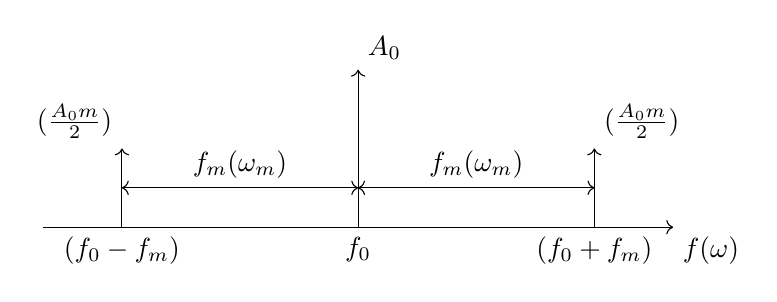
\begin{tikzpicture}
			\draw[->] (1,0) node [below]{$(f_0-f_m)$} -- (1,1) node [above left] {$(\frac{A_0m}{2})$};
			\draw[->] (7,0) node [below]{$(f_0+f_m)$} -- (7,1) node [above right] {$(\frac{A_0m}{2})$};
			\draw[->] (4,0) node [below]{$f_0$} -- (4,2) node [above right] {$A_0$};
			\draw[->] (0,0) -> (8,0) node [below right] {$f(\omega )$};
			\draw[<->] (1,0.5)--(4,0.5);
			\node[align=center, above] at (2.5,0.5) {$f_m(\omega_m)$};
			\node[align=center, above] at (5.5,0.5) {$f_m(\omega_m)$};
			\draw[<->] (7,0.5)--(4,0.5);
		\end{tikzpicture}
		\centering
		\caption{Spectrum of an AM signal, including sidebands}
	\end{figure}

% $A_0$ contains no useful information (bar frequency) which is a disadvantage of Amplitude Modulation.

The simple process of amplitude modulation produces an upper sideband (USB) at $f_0+f_m$ and a lower sideband at $f_0-f_m$. Note that only the sidebands contain any useful information about the amplitude $m$ of the modulation signal.

This modulation has a power penalty because the carrier conveys no useful amplitude information itself.
\begin{eqnarray}
\left(\frac{\mbox{Power in sidebands}}{\mbox{Total power transmitted}}\right) &=& \frac{(0.5A_0m)^2+(0.5A_0m)^2}{(0.5A_0m)^2+(0.5A_0m)^2+A_0^2} \nonumber \\
&=& \frac{0.5A_0^2m^2}{0.5A_0^2m^2 + A_0^2} \nonumber \\
&=& \frac{0.5m^2}{0.5m^2+1}
\label{eqn:power}
\end{eqnarray}

$m = \mbox{modulation depth} = \left(\frac{A_m}{A_0}\right)$ which is a ratio of modulation voltage to the carrier voltage (or current).

It is essential not to let $|m|\ge 1$ because this is overmodulation and it distorts the AM waveform.

Going back to equation \ref{eqn:power}  in the limit $m=1$ and so the ratio is:-
\begin{equation}
\frac{0.5\times 1^2}{(0.5\times 1^2)+1} = \frac{0.5}{1.5} = \frac{1}{3} = 33.3\%
\end{equation}
$\frac{2}{3}$ of the transmitted power is wasted.

Typically, $m\approx 0.4$ from which we have:-
\begin{equation}
\frac{0.5\times 0.4^2}{(0.5\times 0.4^)+1} = \frac{0.08}{0.08+1}
\end{equation}
so this ratio is around 0.08 ie. only 8\% of the transmitted power is used, or 92\% is wasted!

\subsubsection{Waveforms}
	\begin{figure}[h]
		\centering
		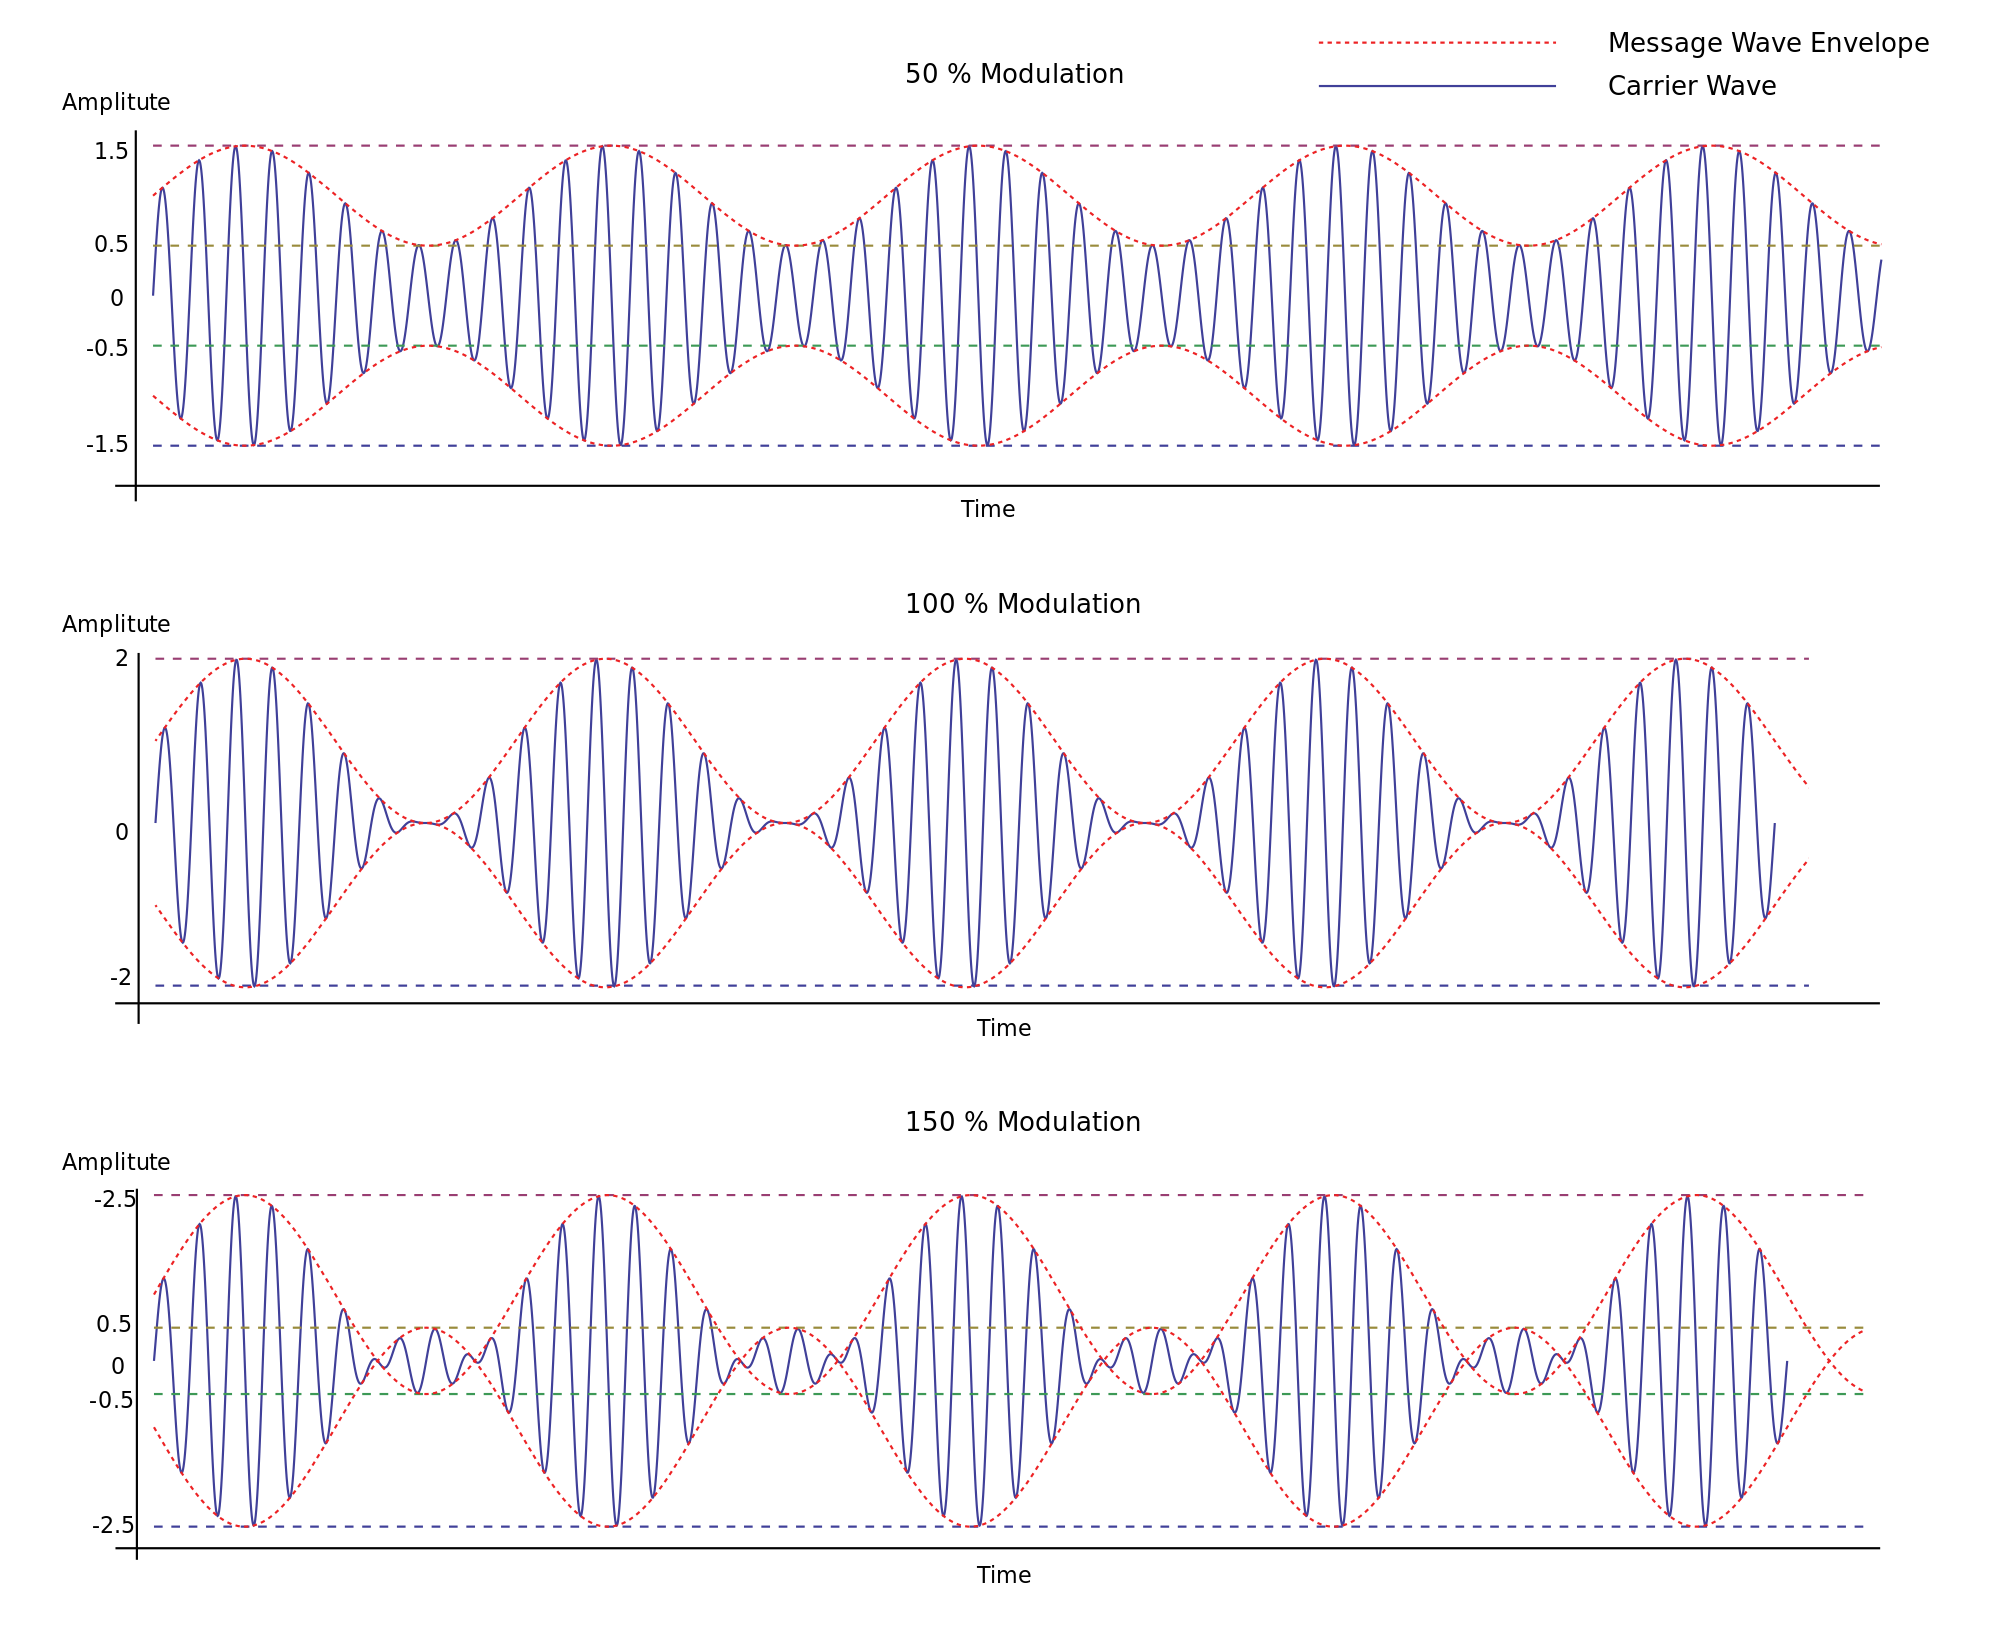
\includegraphics[width=0.8\textwidth]{modulatedwave}
	\end{figure}
It is essential, when considering the above waveform, to have $|m|\le 1$ as mentioned before.

Detecting AM requires an envelope detector in its simplest form:-

\begin{figure}[h]
\centering
\begin{circuitikz}
	\draw
	(0,2) node[anchor=east]{AM input}
	to[D*,o-*] (3,2)
	to[R, l=$R_L$,*-*] (3,0);
	\draw (0,0) to [short,o-*] (3,0);
	\draw (3,2) to[short, *-o] (5.5,2);
	\draw (3,0) to[short, *-o] (5.5,0);
\end{circuitikz}
\caption{Simple envelope detector}
\end{figure}

A more advanced envelope detector adds a low pass filter to remove high frequency components from the carrier wave.
\begin{figure}[h]
\centering
\begin{circuitikz}
	\draw
	(0,2) node[anchor=east]{AM input}
	to[D*,o-*] (3,2)
	to[R, l=$R_L$,*-*] (3,0)
	to[short,*-o] (0,0);
	\draw (3,2) to[short, *-o] (7.5,2);
	\draw (3,0) to[short, *-o] (7.5,0);
	\draw (5.5,0) to[C,*-*] (5.5,2);
\end{circuitikz}
\caption{More advanced envelope detector using smoothing}
\end{figure}

If the carrier frequency is high compared to the modulation frequency, the recovered envelope is a "quite good" approximation to the original given a certain combination of $R_L$ and $C$.


\section{Lecture \ref{sec:lec2} - Double Sideband and Single Sideband AM}
\label{sec:lec2}

	Recall AM signal (Equation \ref{eqn:am}. Power is wasted in the carrier, so a better form of A.M. could be:-
	\begin{equation}
		f(t) = A_0 \cdot \cos{\omega_0} \cdot m\cos{\omega_m t}
	\end{equation}
	Where $m=\frac{A_m}{A_0} = \mbox{modulating depth}$ and $A_m = \mbox{amplitide of modulating signal}$

	\begin{equation}
		f(t) = \left(\frac{A_0m}{2}\right)
		\left(\cos{(\omega_0 +  \omega_m)t}+\cos{(\omega_0 - \omega_m)t}\right)
	\end{equation}

	This is known as double sided sideband, supressed carrier (DSB).

	There is an important property of a DSB $\rightarrow$ for no modulation, no signal is sent, so that it is very power effiicient, but not bandwidth efficient.

	\begin{figure}[h]
		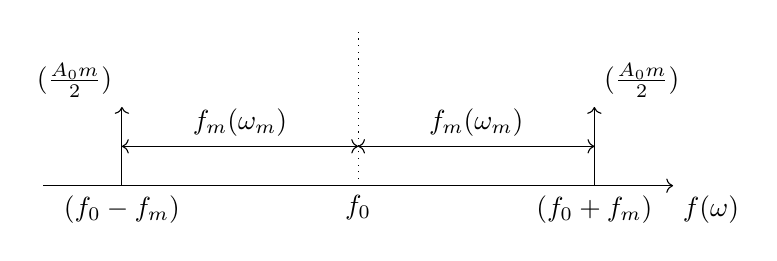
\begin{tikzpicture}
			\draw[->] (1,0) node [below]{$(f_0-f_m)$} -- (1,1) node [above left] {$(\frac{A_0m}{2})$};
			\draw[->] (7,0) node [below]{$(f_0+f_m)$} -- (7,1) node [above right] {$(\frac{A_0m}{2})$};
			\draw[dotted] (4,0) node [below]{$f_0$} -- (4,2);
			\draw[->] (0,0) -> (8,0) node [below right] {$f(\omega )$};
			\draw[<->] (1,0.5)--(4,0.5);
			\node[align=center, above] at (2.5,0.5) {$f_m(\omega_m)$};
			\node[align=center, above] at (5.5,0.5) {$f_m(\omega_m)$};
			\draw[<->] (7,0.5)--(4,0.5);
		\end{tikzpicture}
		\centering
		\caption{Spectrum of a DSB signal}
	\end{figure}


	The envelope of a DSB signal for a single frequency of modulation is:-
	\begin{figure}[h]
		\centering
		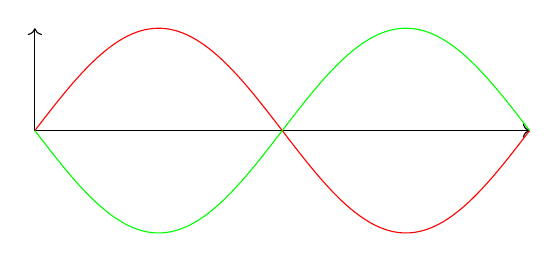
\begin{tikzpicture}[yscale=1.3]
			\draw[<->](0,1) --  (0,0)--(2*pi,0);
			\draw[color=red,domain=0:2*pi,samples=200,smooth] plot (\x,{sin(\x r)});
			\draw[color=green,domain=0:2*pi,samples=200,smooth] plot (\x,{-sin(\x r)});
		\end{tikzpicture}
		\caption{DSB Signal envelope}
	\end{figure}

	Because there is no carrier present, the envelope of the DSB waveform no longer represents the modulating function, therefore an envelope detector cannot be used to detect it - a product detector is used instead.

To illustrate the operation, instead of a DSB being the input, simply use a carrier frequency with no modulation
	\begin{figure}[h]
		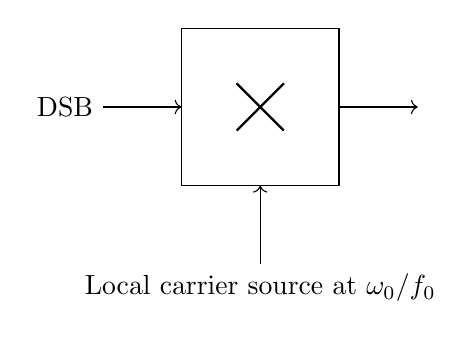
\begin{tikzpicture}
			\draw[->] (0,0) node[left]{DSB} -- (1,0);
			\draw (1,-1) rectangle (3,1);
			\draw[thick, -] ( 1.7,0.3) -- (2.3,-0.3);
			\draw[thick, -] ( 2.3,0.3) -- (1.7,-0.3);
			\draw[->] (2,-2) node[below]{Local carrier source at $\omega_0$/$f_0$} -- (2,-1);
			\draw[->](3,0) --(4, 0);
		\end{tikzpicture}
		\centering
		\caption{Product detector/mixer/multiplexer with simple input}
	\end{figure}

The output after filtering is $\left(\frac{A_0E}{2}\right)$ which is proportinal to $A_0$, the signal amplitude.


		\begin{figure}[h]
		\begin{tikzpicture}
			\draw[->] (0,0) node[ left]{$A_0\cos{\omega_0t}$} -- (1,0);
			\draw (1,-1) rectangle (3,1);
			\draw[thick, -] ( 1.7,0.3) -- (2.3,-0.3);
			\draw[thick, -] ( 2.3,0.3) -- (1.7,-0.3);
			\draw[->] (2,-2) node[below]{$E\cos{\omega_0t}$} -- (2,-1);
			\draw [->](3,0) --(4, 0) node[right]{$A_0\cdot E\cdot \cos^2{\omega_0 t}$};
		\end{tikzpicture}
		\centering
		\caption{Product detector/mixer/multiplexer with real input}
	\end{figure}

Replace the simple input by:-
\begin{equation}
A_0\cos{\omega_0 t} \times \cos{\omega_m t}
\end{equation}
output is
\begin{eqnarray}
(A_0 \times \cos{\omega_0t} \times \cos{\omega_m t})(E\times\cos{\omega_0 t})
&=& A_0 E \cos^2{\omega_0 t}\times\cos{\omega_m t} \\
&=& \left(\frac{A_0 E}{2}\right)(1+\cos{2 \omega_0 t}) \times \cos{\omega_m t}
\end{eqnarray}

After low pass filtering to remove all frequencies above $\omega_m$:-
\begin{equation}
OP = \left(\frac{A_0 E}{2}\right) \times \cos{\omega_m t}
\end{equation}which represent the modulation function directly.

This system can be improved even further because bandwidth is wasted. Bandwidth is important because it is a scarce resource.

If we consider the expanded form of that for DSB:-
\begin{equation}
f(t) = \left(\frac{A_0m}{2} \right) \cos{\left(\omega_0 + \omega_m\right)}t + \left(\frac{A_0m}{2} \right)  \cos{\left(\omega_0 - \omega_m\right)}t 
\end{equation}
If we filter carfully, then we need only send either the USB or LSB.

% Filter image...

Filtering therefore reduces the bandwidth, as each sideband carries the same information (each has an "m" term). Difficulty arises in obtaining sharp cutoff filters. The PHASING METHOD can be used to generate SSB (single side band).

% SSB diagram

\begin{equation}
E_0 = E_1+E_2
\end{equation}

\begin{eqnarray}
E_1 &=& \left[ A_0 \cos{\omega_0 t}\right] \times \left[ \cos{\omega_m t + \frac{\pi}{2}}\right]\nonumber \\
&=& A_0 \cos{\omega_0t}\times \sin{\omega_m t} 
\end{eqnarray}
$\therefore$
\begin{eqnarray}
E_2 &=& A_0 \sin{\omega_0t}\times \cos{\omega_m t}
\end{eqnarray}

$\therefore$
\begin{eqnarray}
E_0 &=& A_0 \times \left[\cos{\omega_0t}\times \sin{\omega_m t}+  \sin{\omega_0t}\times \cos{\omega_m t}\right] \nonumber \\
&=& A_0 \sin{\left(\omega_0 + \omega_m\right)} t
\end{eqnarray}
USB, no filtering needed.

Similarly, the LSB can be generated by changing the sign of the second term above (on the first term).

The method works very well only when a single frequency of modulation is used. In practice, a range of frequencies is used and it is very difficult to obtain a 90\textdegree phase shift over a range of frequencies.

\subsection{Vestigial Sideband}
Remember all the abbreviations, "in case they get slipped into a question"
This is an approximation to SSB which has been used extensively in analogue T.V. ver many decades. Basically, a DSB/C (Double Sideband with Carrier)

% Vestigial sideband plot...

The main benefits are: simplicity and cheapness compared to SSB, when using valve/vacuum tube technologies.

The disadvantage is carrier still there, wasting power, but allowing an envelope detector (cheap, easy to make) to be used.

\section{Lecture 3 - Angle Modulation}
Starting with \ref{eq:rf}
\begin{equation}
f(t) = A_0 \cdot \cos\left(\omega_0t+\phi\right)
\end{equation}

In the expression for $f(t)$ if we make $(\omega_ct+\phi)=\phi(t)$ then $\phi_c$ may be made instantaneously proportional to the modulating signa $f_m(t)$:-
\begin{eqnarray}
\phi\left(t\right) &=&  \omega_ct+k_p f_m(t) \nonumber \\
\implies f(t) &=& A_0 \cos\theta(t)
\end{eqnarray}
where $k_p = \mbox{constant of modulation}$. This is Phase Modulation.

Alternatively, we can have 
\begin{eqnarray}
	\omega(t) &=& \left[\frac{d\phi(t)}{dt}\right] \nonumber \\
	&=& \omega_c + k_f \cdot f_m(t)
\end{eqnarray}
where, as before $k_f$ is a constant.

In this case, the instantaneous frequency has the value $\omega_c$ in the absence of a modulating signal. By integrating the above expression $\frac{d\theta(t)}{dt}$:-

\begin{eqnarray}
\omega(t) &=& \frac{d\theta(t)}{dt} \implies \int{\omega(\theta)}dt = \theta(t) \nonumber \\
\implies \theta(t) &=& \omega_ct + k_f \int{f_m(t)} dt + \phi_0
\end{eqnarray}
This is frequency modulation.

Frequency modulation is thus an indirect form of pulse modulation and is mathematically related.

% Diagram

Phase and frequency modulation are thus similar in form and are both angle modulation.

Frequency modulation can be generated easily using a voltage controlled oscillator.

% VCO diagraom

\subsection{Detection of FM}
An FM discriminator (or Phase Locked Loop) is used to convert frequency changes to amplitude changes:-
% Frequency graph
\begin{figure}
	\begin{tikzpicture}[yscale=0.5,xscale=1]
		\draw[->]  (-4,0) -- (4,0) node[below]{Frequency};
		\draw[->]  (0,-4) -- (0,4) node[left]{Amplitude};
		\draw[blue] (-3,-2) -- (-2,-3) -- (2,3) -- (3,2);
		\draw[dotted](-2,0) node[above]{$(f_0-f_{max})$} -- (-2,-3);
		\draw[dotted](2,0) node[below]{$(f_0+f_{max})$} -- (2,3);
	\end{tikzpicture}
\centering
\caption{FM spectrum usage}
\end{figure}
At frequency $f_0$ the output of the FM demodulator is zero. For frequencies above $f_0$ (but less than $\pm f_{max}$ then the output is greater than zero (or inverted and greater than 0 for $f < f_0$. The output of such a discriminator is then fed to a circuit or system which detects amplitude changes.

F.M. and P.M. generate a different spectrum to let $f_m(t) = \cos{\left(\omega_mt\right)}$ for F.M.
\begin{eqnarray}
\therefore f(t) &=& A_0 \cdot \cos{\left[\omega_0t + k_f\int^t_0\cos{\left(\omega_mt\right)}dt\right]} \nonumber \\
&=& A_0\cdot\cos{\left[\omega_0t+\left( \frac{k_f}{\omega_m}\right)\sin{\omega_mt }\right]}
\end{eqnarray}

The instantaneous frequency of this value is $f_i = \frac{(\omega_0 +k_f\cos{\omega_mt})}{2\pi}$ which oscillates between two extreme values:-
\begin{equation}
\left[ \frac{\omega_0}{2\pi} \right] \pm \left[ \frac{k_f}{2\pi} \right] \mbox{for } cos(\omega_mt)_max=\pm 1
\end{equation}

The peak value of the difference between $f_i$ and the carrier frequency $f_0 = \left( \frac{\omega_0}{2\pi}\right)$ is the frequency deviation, which is $\left[ \frac{k_f}{2\pi}\right]$ in the above example.

% Real might be the wrong word here...
Since $k_f$ is proportional to the real amplitude of the modulating signal, so is the frequency deviation.

If $f_d$ is the maximum frequency deviation and $f_a$ is the actual frequency deviation then the deviation ratio, $m$ is defined as:-
\begin{equation}
m=\frac{f_a}{f_d}
\end{equation}
Now $f_a = \frac{k_f}{2\pi}$ so $m=\left[\frac{k_f}{2\pi\cdot f_d}\right]$
$\therefore$ 
\begin{equation}
\left(\frac{k_f}{\omega_m}\right) = \frac{2\pi f_a}{2\pi f_m} = \frac{f_a}{f_m} = m\frac{f_d}{f_m}
\end{equation}

(Comparing actual frequency deviations to the modulating frequency $f_m$).
\begin{eqnarray}
\implies \frac{mf_d}{f_m} &=& m_p = \mbox{modulation index} \nonumber \\
\therefore f(t) &=& A_0 \cdot\cos{\left[\omega_0t+m_p\cdot\sin{\omega_mt}\right]}
\end{eqnarray}

Usign Bessel functions, 
\begin{equation}
	f(t) = A_0 \sum_{m=\infty}^{\infty}{I_n(m_p)\cdot \cos{(\omega_c + n\omega_m)}t}
\end{equation}
therefore firstly, FM thus generates a range of frequencies from $-\infty$ to $\infty$ in practice, the bandwidth is restricted and also the Bessel coefficient ($=I$) have finite values which tend to zero as n tends to $\pm \infty$

\begin{table}[h]
    \begin{tabular}{cccc}
        \hline
 & & \multicolumn{2}{c}{Bandwidth}  \\
Modulation Index $m_p$ & No. of sidebands $n$ &  (a) as multiples of $f_m$ & (b) as multiples of $f_a$ \\ \hline
	0.1 &  2 & 2 & 20 \\
	0.5 & 4 & 4 & 8 \\
	1 & 6 & 6 & 6 \\
	5 & 16 & 16 & 3.2 \\
	30 & 70 & 70 &2.3 \\
    \end{tabular}
	\caption{Modulation index to bandwidths}
	\label{tab:modind}
\end{table}

\section{Lecture 4}
\begin{equation}
B = n\cdot f_m = N\cdot\left(\frac{f_a}{mp}\right)
\end{equation}
Where $f_a=$ frequency deviation and $f_M$ = modulating frequency.

E.g: For VHF/FM mono transmissions, the maximum value of $f_a=75\mbox{kHz}$ and the maximum value of $f_m=15\mbox{kHz}$ (speech and music quality).
therefore $m = \frac{f_{a(max}}{f_{m(max)}} = 5$. Looking at table \ref{tab:modind} above, we can see that, for $m=5$ we need a bandwidth of $(3.2\times 75\mbox{kHz})=240\mbox{kHz}$. The reason why such a large bandwidth is needed is because F.M. causes the frequency changes to occur at a high rate, resulting in a much larger change in spectrum.

\subsection{Zenith-GE FM Stereo System}
The FM stereo signal has to have backwards compatibility with mono, and uses independent left ($L$) and right ($R$) signals. When a mono source is used, the stereo signal has to revert to a mono representation for backward compatibility. Conversely, when a stereo signal is received by a mono receiver, then the latter should be able to interpret the stereo as a mono source (forward compatibility).

The L and R signals are formatted at the transmit end into ($\underbrace{L+R}_{\mbox{\scriptsize mono}}$) and ($\underbrace{L-R}_{\mbox{\scriptsize "stereo"}}$).

The Zenith stereo signal, overall, uses both of the above. The ($L+R$) signal is baseband, and the ($L-R$) signal is used with DSB/SC (AM) at $38kHz$:-

\begin{figure}[h]
	\centering
	\begin{tikzpicture}[xscale=0.25]
		\draw[<->] (0,4) node[left]{Amplitude}--(0,0)--(56,0) node[below]{$f$};
		\draw (0,3) -- (15,3) -- (16,0);
		\draw[dotted] (15,0) node[below]{$15kHz$}--(15,3);
		\draw[green] (23,0) -- (24,2.9) -- (37,2.9) -- (38,0) node[below] {$38kHz$}-- (39,2.9) -- (52, 2.9) -- (53,0);
		\draw[->,blue,dotted](19,0)node[below, text width=1cm,align=center]{$19kHz$ pilot tone} -- (19,1.8); 
		\draw (55,3)node[above] {DSB/SC};
	\end{tikzpicture}
	\label{fig:zenith}
	\caption{Zenith-GE spectrum}
\end{figure}
The "pilot tone" is used a the receiver to generate $38kHz$ at the correct phase so as to be able to demodulate the ($L-R$), DSB/SC signal optimally. The ($L-R$) and pilot tone signals have to be constrained in amplitude to prevent "over modulation" of the FM carrier and this prevent distortions and consequent unwanted frequencies being generated. Typically, ($L-R$) is limited to 45\% of  its maximum value, in which case the overall signal (i.e. ($L+R$), pilot tone and ($L-R$)) never exceeds 90\% of the overall possible maximum amplitude. Note that ($L+R$) can be recovered directly by using a $15kHz$ low pass filter (LPF) at the receiver -- which is the mono component, and can be easily interpreted by a mono receiver.

The ($L-R$) signal must be recovered using a $38kHz$ signal derived from the $19kHz\left(=\frac{38}{2}\right)$ pilot tone as mentioned. The base bandwidth of the stereo signal is $53kHz$ (from figure \ref{fig:zenith})

Using Carson's Rule (an approximation), we can calculate the required overall FM bandwidth as
\begin{equation}
B = 2 \cdot \left[f_{a(max)}+f_{m(max)}\right]
\end{equation}
where $f_{a(max)} = 75kHz$ (to be compatible with mono) $f_m(max) = 53kHz$, therefore $B=256kHz$.

FM has a SNR (signal to noise ratio) advantage over AM above a crtical threshold. Below the threshold the FM signal becomes unusable very quickly. FM as above is a simple form of "spread spectrum".
\end{document}